\documentclass[tikz,border=10pt]{standalone}
\usetikzlibrary{angles,calc,intersections}
\begin{document}
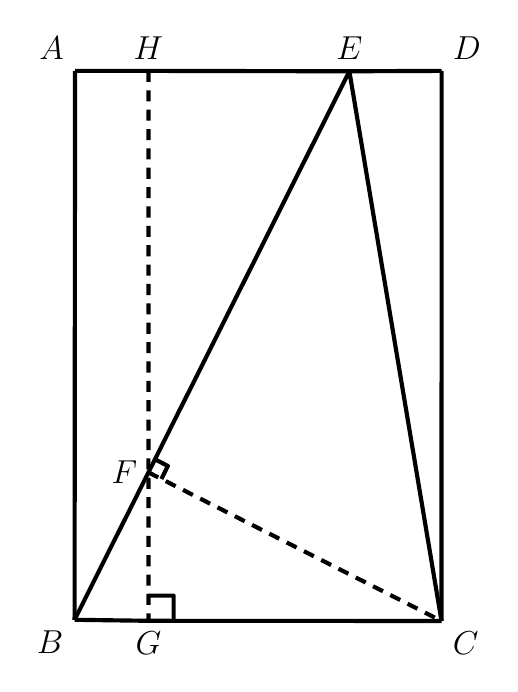
\begin{tikzpicture}[line width=1.5pt, line join=round]
\coordinate (A) at (-2.337,3.501);
\coordinate (B) at (-2.343,-3.470);
\coordinate (C) at (2.317,-3.485);
\coordinate (D) at (2.319,3.501);
\coordinate (G) at (-1.405,-3.483);
\coordinate (H) at (-1.405,3.501);










\coordinate (E) at (1.147,3.496);


\coordinate (F) at (intersection of B--E and H--G);


\draw (A) -- (B);
\draw (A) -- (H) -- (E) -- (D);
\draw (D) -- (C);
\draw (B) -- (G) -- (C);


\draw (B) -- (E) -- (C);


\draw[dash pattern=on 4pt off 3pt] (H) -- (F) -- (G);
\draw[dash pattern=on 4pt off 3pt] (F) -- (C);


\draw pic[draw, angle radius=0.185cm] {right angle=E--F--C};
\draw pic[draw, angle radius=0.320cm] {right angle=C--G--H};



\node[above left, font=\fontsize{13}{15.6}\selectfont] at (A) {$A$};
\node[above, font=\fontsize{13}{15.6}\selectfont] at (H) {$H$};
\node[above, font=\fontsize{13}{15.6}\selectfont] at (E) {$E$};
\node[above right, font=\fontsize{13}{15.6}\selectfont] at (D) {$D$};
\node[left, font=\fontsize{13}{15.6}\selectfont] at (F) {$F$};
\node[below left, font=\fontsize{13}{15.6}\selectfont] at (B) {$B$};
\node[below, font=\fontsize{13}{15.6}\selectfont] at (G) {$G$};
\node[below right, font=\fontsize{13}{15.6}\selectfont] at (C) {$C$};
\end{tikzpicture}
\end{document}